\documentclass[a4paper]{article}

%% Language and font encodings
\usepackage[english]{babel}
\usepackage[utf8x]{inputenc}
\usepackage[T1]{fontenc}

%% Sets page size and margins
\usepackage[a4paper,top=3cm,bottom=2cm,left=3cm,right=3cm,marginparwidth=1.75cm]{geometry}

%% Useful packages
\usepackage{amsmath}
\usepackage{graphicx}
\usepackage[colorinlistoftodos]{todonotes}
\usepackage[colorlinks=true, allcolors=black]{hyperref}
\usepackage{comment}
\usepackage{url}

% Code
\usepackage{listings}

\begin{document}

\newcommand{\customlarge}[1]{\noindent \Large{\textbf{#1}}}
\newcommand{\customitalic}[1]{\large{\textbf{\textit{#1}}}}
\newcommand{\avis}[2]{\customlarge{Avis personnel -} \customitalic{#1} \\ #2\\[0.8cm]}
\newcommand*{\escape}[1]{\texttt{\textbackslash#1}}

\newcommand{\customquote}[1]{\guillemotleft {#1} \guillemorright~}

\renewcommand{\contentsname}{Sommaire}

\begin{titlepage}
\newcommand{\HRule}{\rule{\linewidth}{0.5mm}} % Defines a new command for the horizontal lines, change thickness here

\center % Center everything on the page
 
%----------------------------------------------------------------------------------------
%   HEADING SECTIONS
%----------------------------------------------------------------------------------------

\textsc{\LARGE Université de Bordeaux}\\[0.5cm]
\textsc{\large Département Informatique}\\[0.5cm]
\textsc{\large Année 2019-2020}\\[1.5cm]
\textsc{\Large Groupe 21-2}\\[0.2cm] 
\textsc{\large Master 1}\\[0.3cm] 

%----------------------------------------------------------------------------------------
%   TITLE SECTION
%----------------------------------------------------------------------------------------

\HRule \\[0.4cm]
{  \huge \bfseries Projet de Programmation: \\
   \huge \bfseries Génération procédurale de planètes sphériques\\[0.4cm] 
   \Large \bfseries Analyse des besoins
% Title of your document
\HRule \\[1.5cm]
 
%----------------------------------------------------------------------------------------
%   AUTHOR SECTION
%----------------------------------------------------------------------------------------

\begin{minipage}{0.4\textwidth}
\begin{center} \large
\emph{Client:}\\
David \textsc{Renault}\\
~\\
\emph{Auteurs:}\\
Rémi \textsc{Barbosa}\\
Benjamin \textsc{Darmet}\\
Marc \textsc{Cerutti}\\
Sofian \textsc{Antri}\\
Tsiory \textsc{Rakotoarisoa}\\
\end{center}
\end{minipage}
~
}

% If you don't want a supervisor, uncomment the two lines below and remove the section above
%\Large \emph{Author:}\\
%John \textsc{Smith}\\[3cm] % Your name

%----------------------------------------------------------------------------------------
%   DATE SECTION
%----------------------------------------------------------------------------------------

% {\large \today}\\[2cm] % Date, change the \today to a set date if you want to be precise

%----------------------------------------------------------------------------------------
%   LOGO SECTION
%----------------------------------------------------------------------------------------


%----------------------------------------------------------------------------------------

\vfill % Fill the rest of the page with whitespace

\end{titlepage}

% ------------------------ END OF TITLEPAGE ------------------------
\newpage

\tableofcontents

\newpage

\section{Présentation du projet}

\paragraph{}
Les besoins en détails et en tailles des mondes virtuels étant toujours plus grands, l'automatisation de contenu numérique est devenu un enjeu véritablement important. C'est alors que la génération procédurale fit son apparition. En informatique, la génération dite procédurale est la création de contenu numérique (modèle 3D, animation, son, musique,...) à une très grande échelle et en grande quantité, de manière automatisée. Elle doit répondre à un ensemble de règles qui sont définies par des algorithmes.
\paragraph{}
Nous cherchons à mettre en place au sein de ce projet, un outil permettant de générer procéduralement et de visualiser des planètes (une à la fois) dans un but ludique (se balader pour le plaisir d'admirer et explorer, découvrir un nouvel environnement). Chaque planète est représentée par une sphère géodésique (divisée en faces) statique dont les faces colorées témoignent de la présence de différent terrains, tels que des océans, des reliefs, des déserts, des plaines etc. La planète aura un rendu "low-poly", désignant un style graphique, souvent utilisé dans le développement de jeux-vidéo, avec peu de polygones et donc volontairement peu de détails pour des raisons d'optimisation mais aussi d'esthétique. Une fois la planète généré, il sera possible de la visualiser par une vue à 360° en orbite autour de la planète. Cette vue s'accompagnera d'un outil de zoom afin d'obtenir par la suite une fois très proche, un changement d'orientation du plan pour pouvoir observer l'horizon en première personne, vue humaine, sans déplacement.

\begin{figure}[!h]
\begin{center} 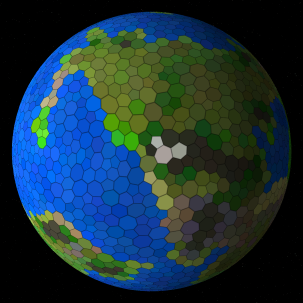
\includegraphics{img/planete.png} \end{center}
\caption{Exemple de planète générée procéduralement}
\end{figure}

\newpage
\section{Analyse de l'existant}

\subsection{Algorithmes de génération de sphère}

Il existe différentes méthodes pour générer une sphère à face polygonale. Il est possible soit de subdiviser un icosahedron (polyèdre à 12 sommets et 20 triangles équilatérals) à plusieurs reprises, ou d'utiliser une sphère de Fibonacci (Mettre ref.).En utilisant la sphère de Fibonnaci, il est néanmoins plus compliquer de mettre en place les faces polygonales. En effet, il s'agit uniquement de dispersion de points formant une sphère. Mais ces points ne sont pas reliés. Il est alors nécessaire d'utiliser des techniques qui permettent cela. Les plus connus sont : "la triangulation de Delaunay" et "les régions de Voronoi". \cite{RedBlobGames}
\newline
Dans le cas de l'icosahedron, chaque triangle est divisé en 4 sous-triangles égaux jusqu'à l'affinage souhaité.
\newline
Au vu de la complexité d'utilisation des deux méthodes présentées ci-dessus avec une sphère de Fibonnaci, la technique de la subdivision est recommandée. 

\subsection{Outils existants et prototypes}

\subsubsection{Blender}

Afin de pouvoir générer et afficher notre planète, une des solutions qui peut-être abordé est l'utilisation d'outils de modélisation 3D, ayant du coup déjà des moteurs de rendus performant, dont certains utilisent un système de scripting et de plugin afin de générer des formes, les modifier, et les texturer, pour ensuite les utiliser plus tard dans d'autres logiciels aussi selon des formats standardisé.
L'un de ces outils existant est l'outil Blender. Il est tout d'abord un logiciel open Source, dont le moteur interne est en C/C++ permettant de bonnes performances. Il dispose aussi une API en Python permettant un prototypage très rapide.
\\\\
Nous avons du coup fait un script Python qui en soit :
\begin{itemize}
            \item {créer une icosphére d'environ 10 000 polygones au moins.}
            \item {application d'une transformation sur ses sommets selon une texture de Voronoi.}
            \item {Affiches les paramètres et le temps de génération.}
\end{itemize}

Vous pouvez retrouver le script dans la hiérarchie du projet \textit{docs/requirements/test\_blender}, et les résultat. Le premier résultat obtenu en exportant l'image depuis l'éditeur est ci-dessous :
\begin{figure}[!h]
\begin{center} 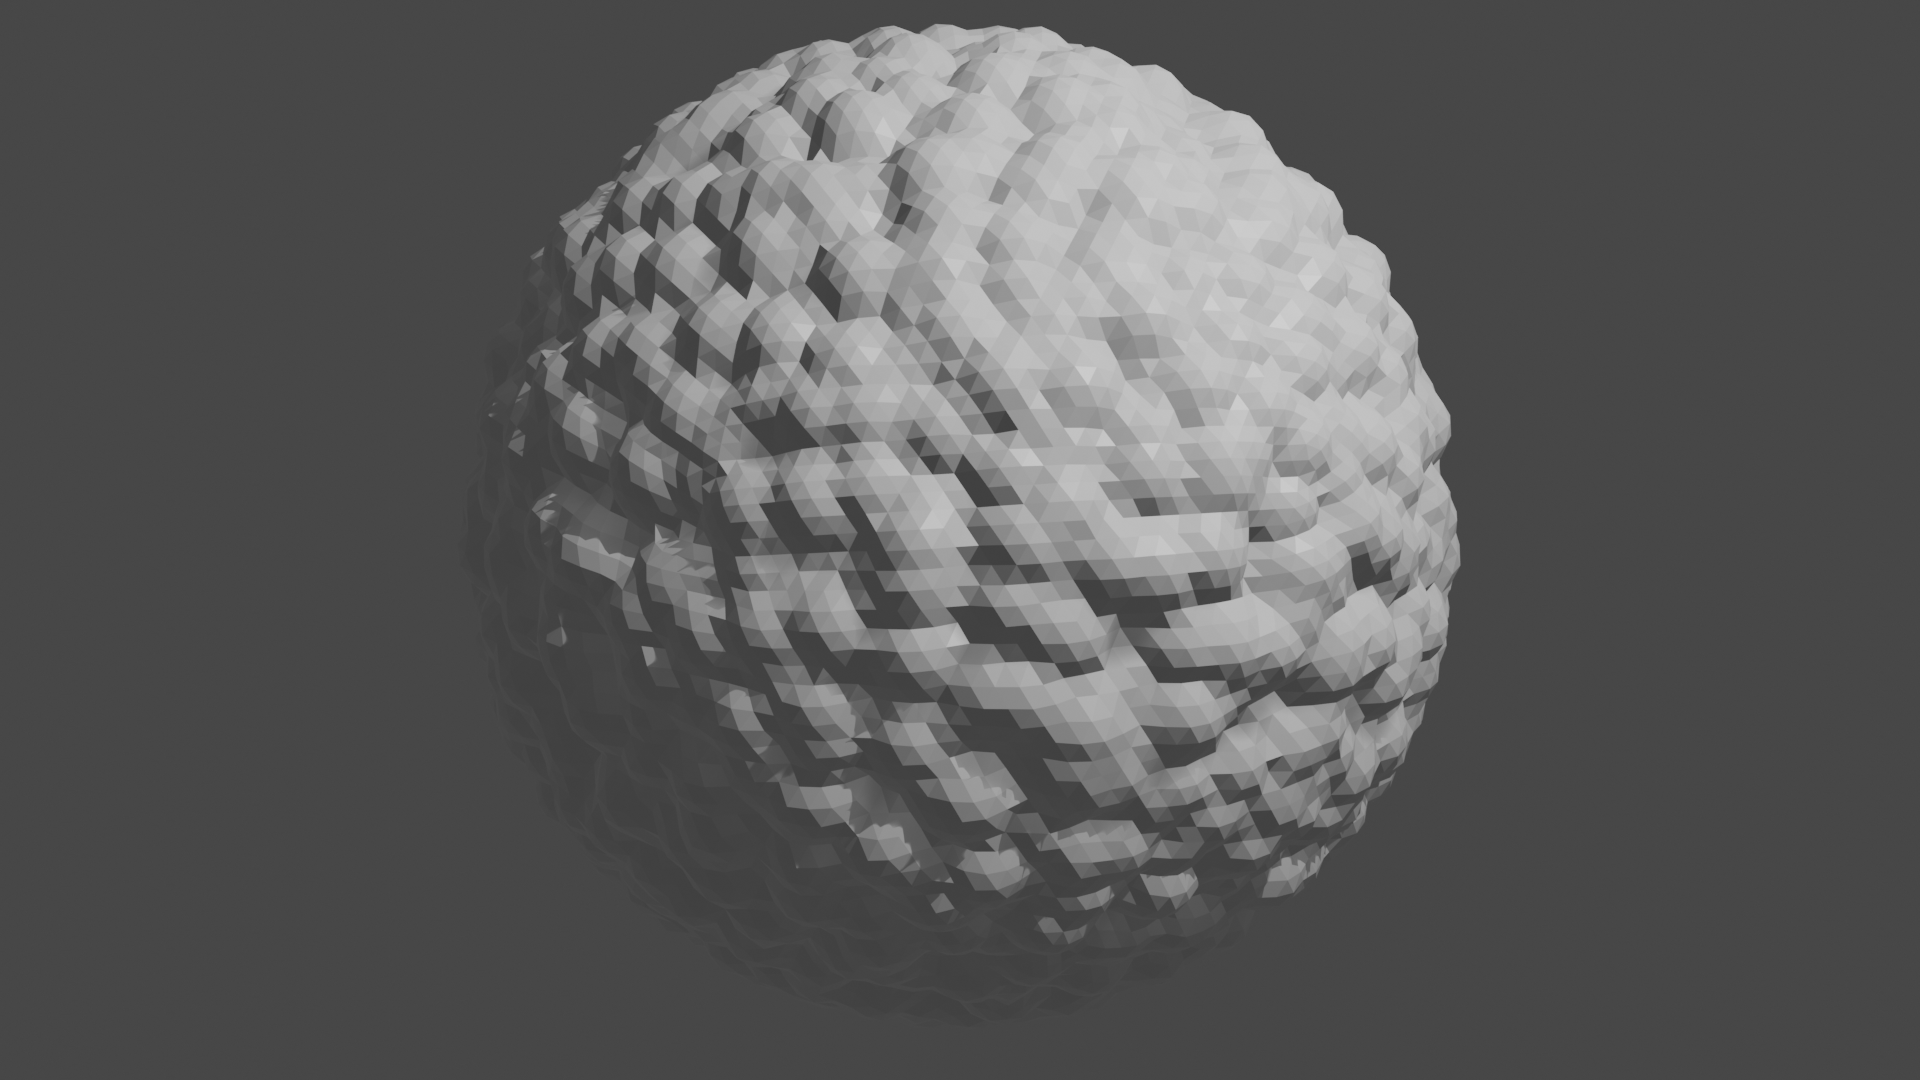
\includegraphics[width=0.5\linewidth]{img/blender_1.png} \end{center}
\caption{Icosphère généré par Blender. Texture de bruit Voronoï, 6 subdivision, \textasciitilde0.02 s, 20480 polygones}
\end{figure}

Attention par contre à la version de Blender, nous avons utiliser le moteur de rendu Evee de la version 2.8 permettant une visualisation sans perte de Fps lors des opérations de manipulation de de la visualisation (rotation, zoom) avec les rendus finaux. Il faut aussi faire attention à la machine utilisé et notamment la carte graphique.\\
Nous avons pu ensuite en changeant les paramètres depuis l'éditeur blender arriver aux résultat suivant.

\newpage
\begin{figure}[!h]
\begin{center} 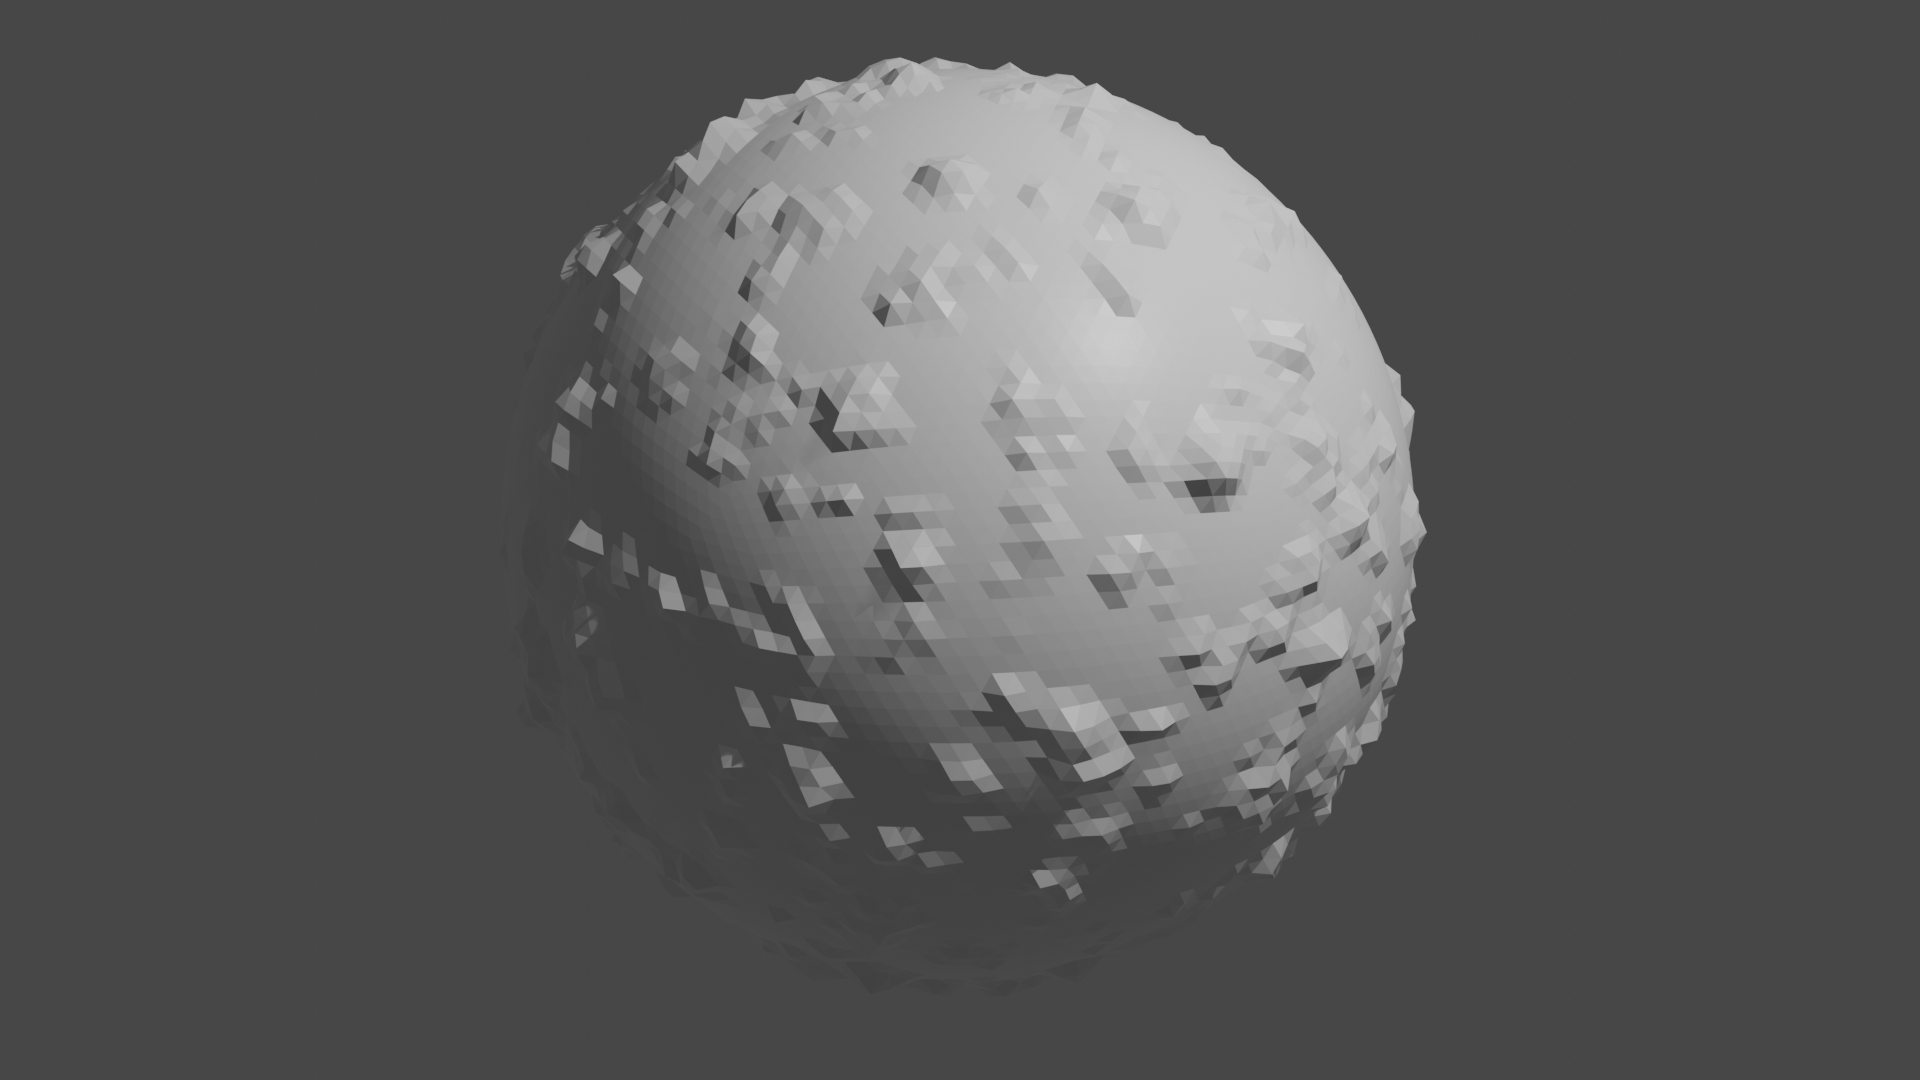
\includegraphics[width=0.5\linewidth]{img/blender_2.png} \end{center}
\caption{Modification de texture bruit de déplacement Voronoï sans couleur}
\end{figure}

\begin{figure}[!h]
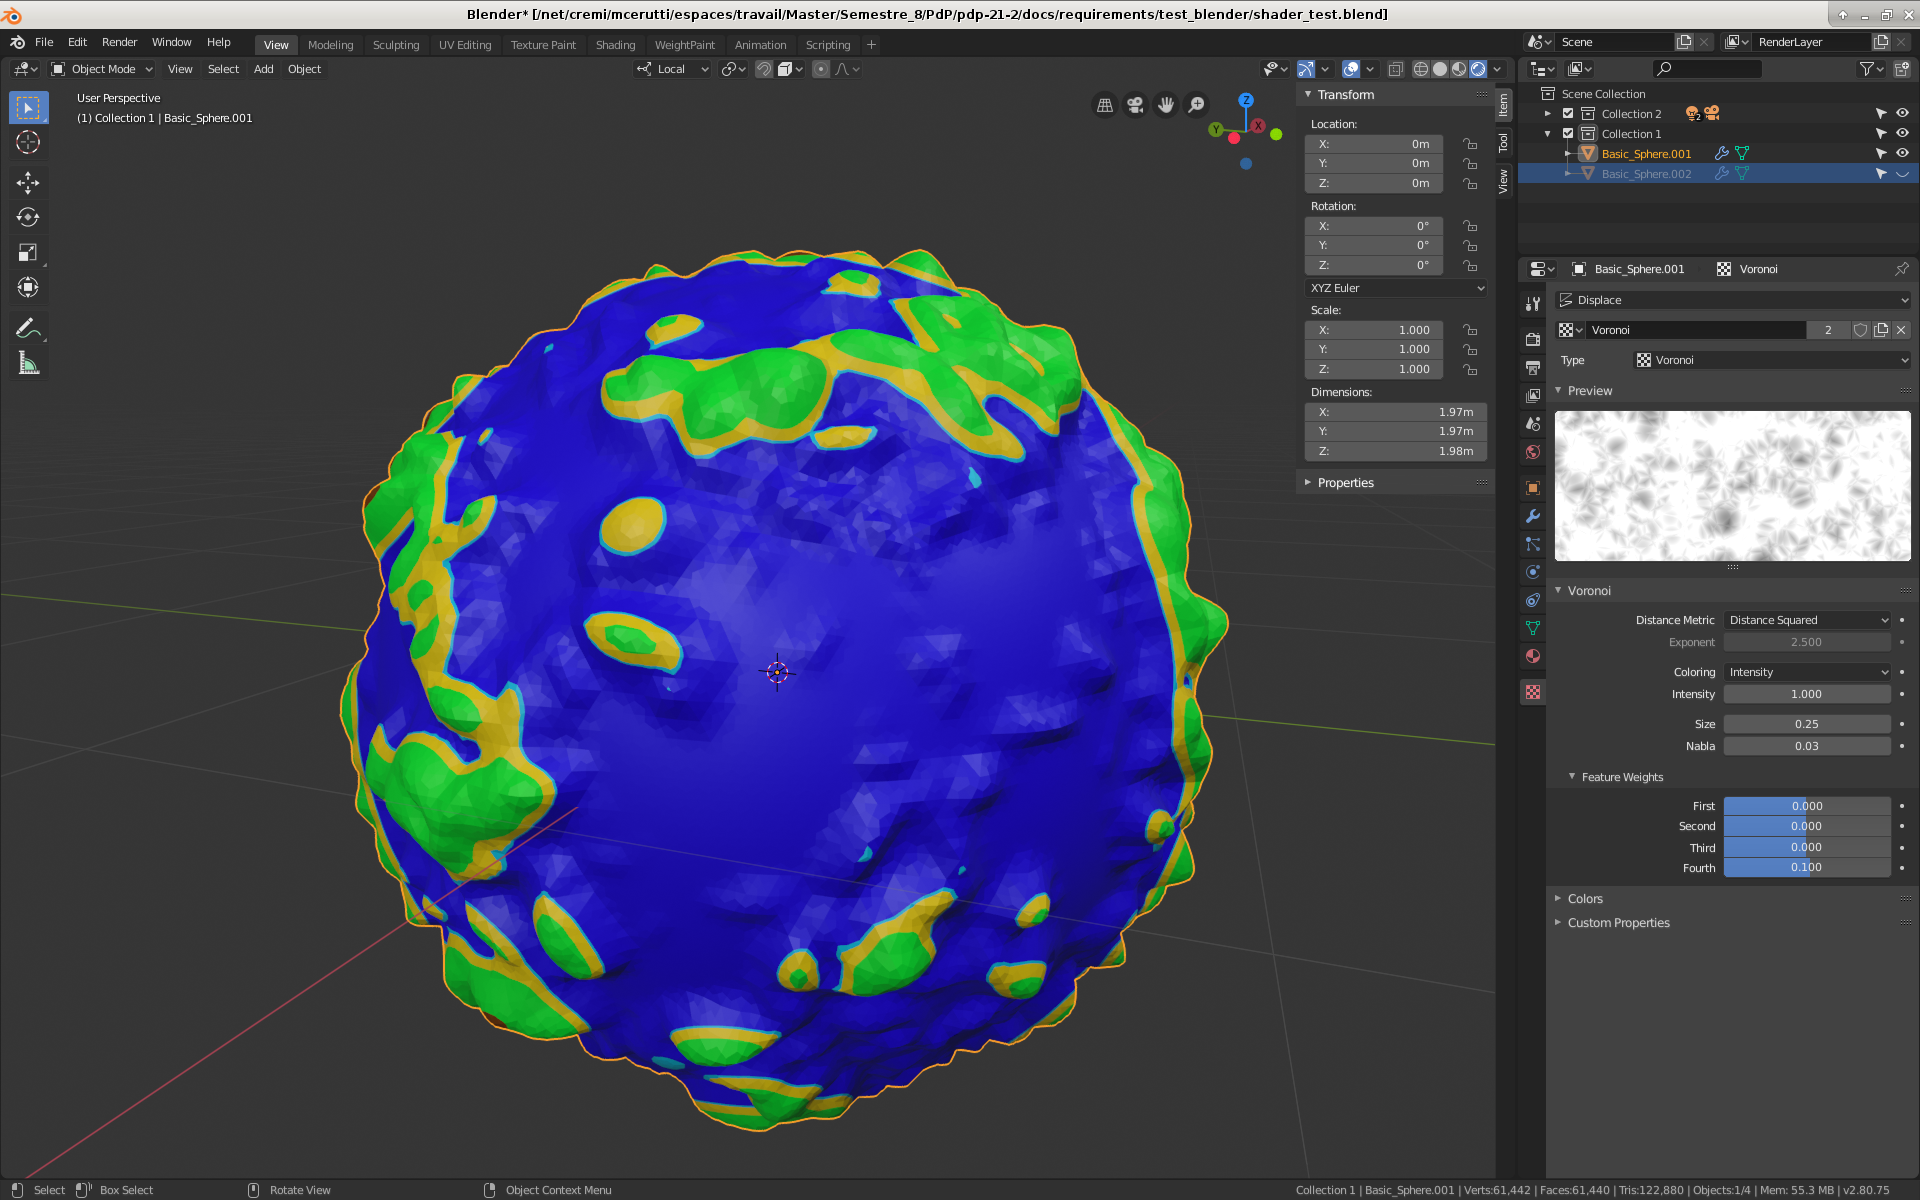
\includegraphics[width=0.49\linewidth]{img/blender_editeur_bruit.png}
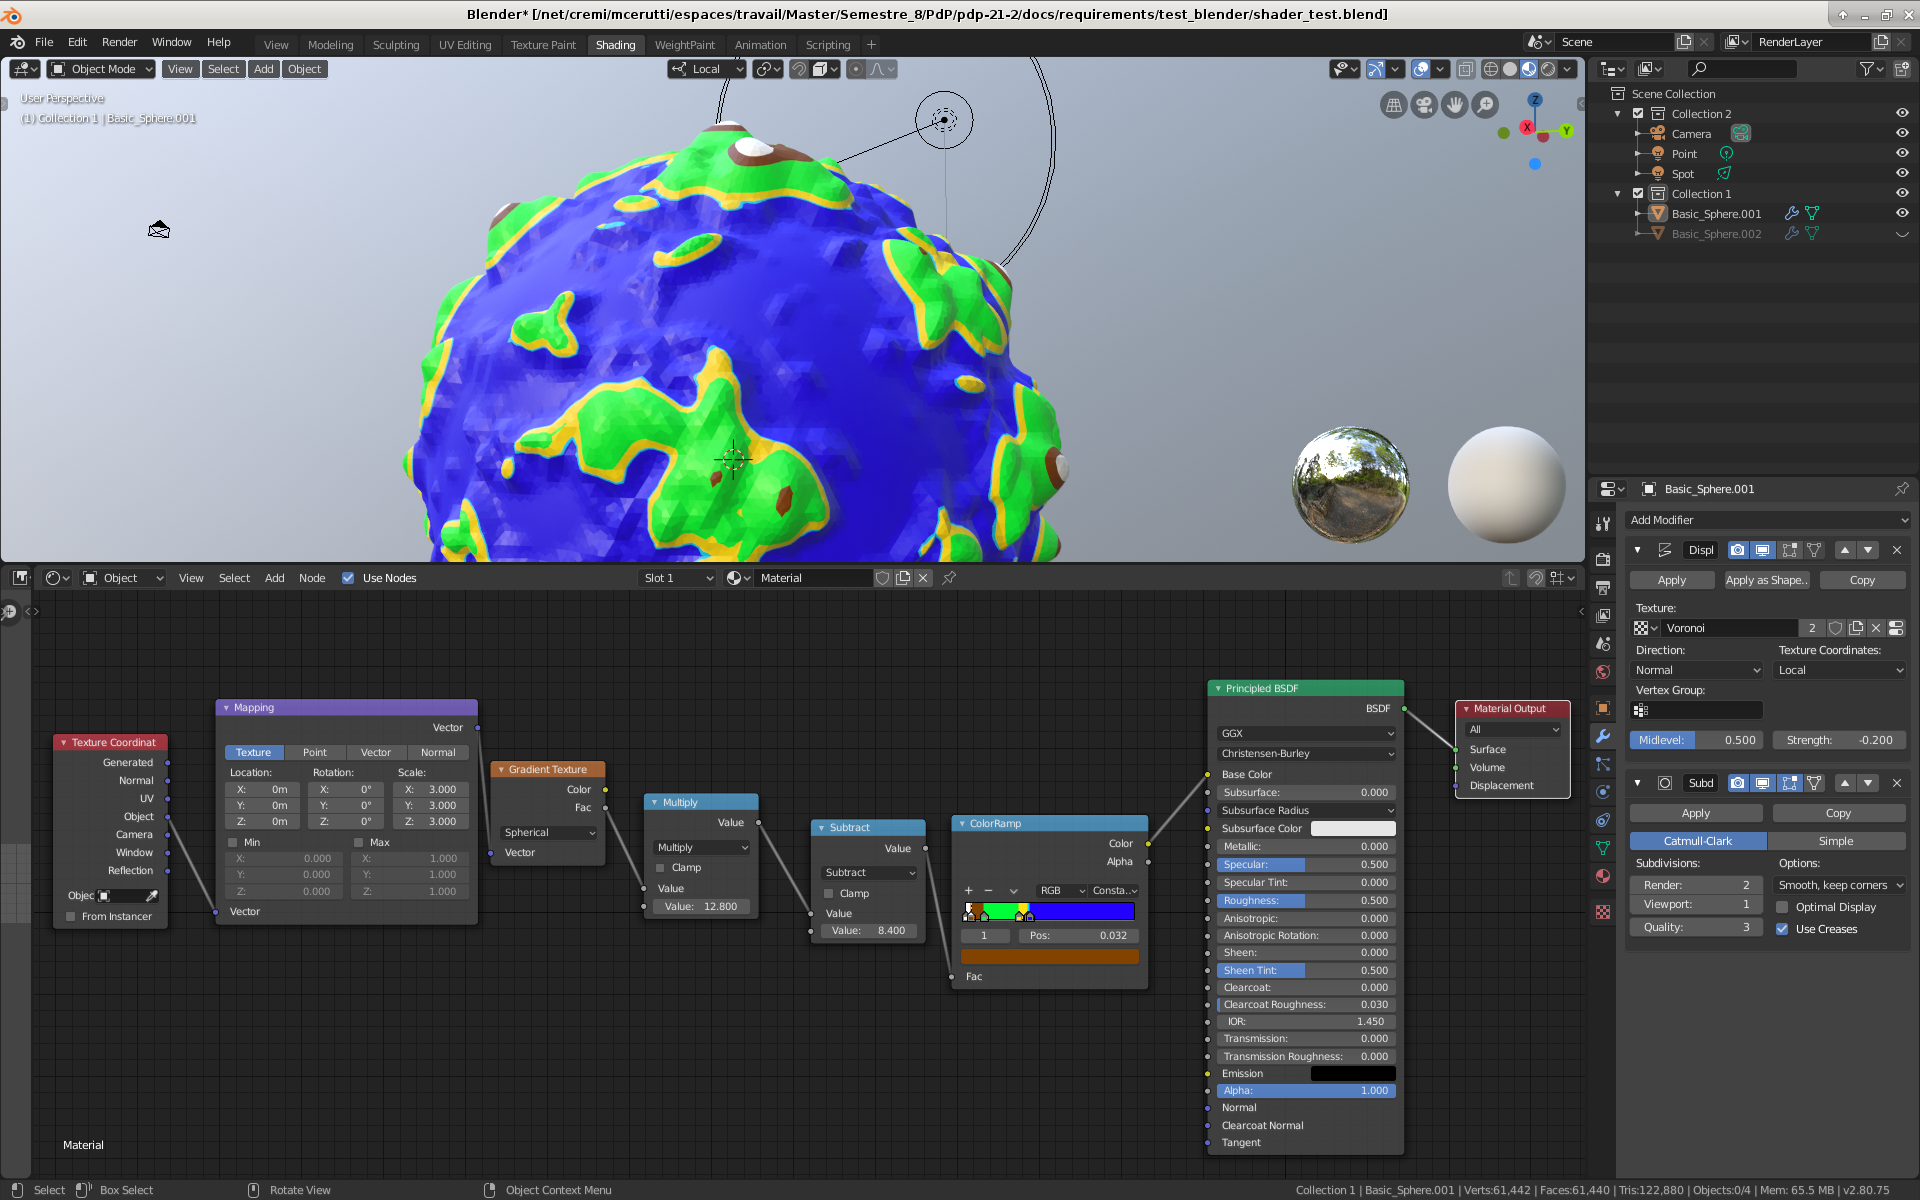
\includegraphics[width=0.48\linewidth]{img/blender_shaderEditor.png}
\caption{Essais de modifications par l'éditeur Blender : Paramètres de texture, bruit de déplacement des vertices, rajout de shader}
\end{figure}

\paragraph{Avantages}

\begin{itemize}
            \item {Rendu de base avec OpenGL, Moteur interne en C/C++.}
            Permet d'espérer de très bonne performances au niveau des algorithmes de base. Crucial dans le cas de rendu de l'ordre de 60 FPS avec une bonne machine.
            \item {Opensource et libre de droit.}
            Cela nous permettrai de modifier le moteur de rendu, et les algorithmes de visualisation selon nos besoins.
            \item {Crossplatform.}
            Permet le portage Linux, et aussi sur d'autres plateformes nativement.
            \item {API très simple en Python afin d'accéder et de modifier la forme.}
            Permet de faire des tests très rapide, et de manipuler par le client les algorithmes de modifications plus facilement qu'on aurait implémenté en surcouche du moteur interne.
            \item {Fonctionnalités supplémentaire (sauvegarde, modification, amélioration de rendu, création de shader en node...)}
            Permettrai de se concentrer sur les fonctionnalités intéressantes en ayant déjà les possibilités d'extensions de notre projet.
\end{itemize}

\paragraph{Inconvénient}

    \begin{itemize}
                \item {Interface de blender trop riche pour le client.}
                Contraire à la demande du client que la visualisation soit simple. Nécessite une connaissance au moins de surface de l'outil. Risque de refus à envisager avant de commencer à l'utiliser.
                
                \item {Rendu et génération dépendant de la machine choisi.}
                En soit c'est un risque difficilement évitable peu importe l'outil envisagé. On doit du coup demander la configuration au client.
                
                \item {La version de Blender influe sur l'API (2.8 non documenté formellement encore), et sur les performances de rendu (moteur Evee).}
                Risque de bug sur l'API fourni et d'instabilité. A voire par rapport au niveau de sécurité voulu par le client. Risque aussi d'un développement plus chaotique du fait du manque de documentation.
                
                \item {Pas de sécurité sur des paramètres trop grand (cesse de fonctionner, pas d'erreurs de ressources si demande trop grande).}
                Lié au fait d'utiliser une API en "boîte noir", nécessite un apprentissage des fonctions du moteur interne et une bonne documentation. Cela aussi influe sur la flexibilité du code et les limites d'extensions avec le logiciel de base..
                
    \end{itemize}

\subsubsection{OpenGL}
OpenGL(Open Graphics Library) est considéré comme une API en  qui offre la capacité d'afficher des objets en 2D et en 3D et est principalement utilisé pour interagir facilement avec les cartes graphiques (GPU). Néanmoins, c'est avant tout une spécification, qui décrit ce que sont les entrées et sorties de chaque fonction et comment elles doivent s'exécuter. C'est alors au développeur d'implémenter ces fonctions. Il est alors nécessaire d'utiliser une librairie (principalement écrite par les constructeurs de carte graphique). La version 3.3 quant à elle, permet une grande flexibilité et efficacité. Il est ainsi possible d'afficher une sphère de plus de 10 000 polygones, comme le prouve la figure ci-dessous.


\begin{figure}[!h]
\begin{center}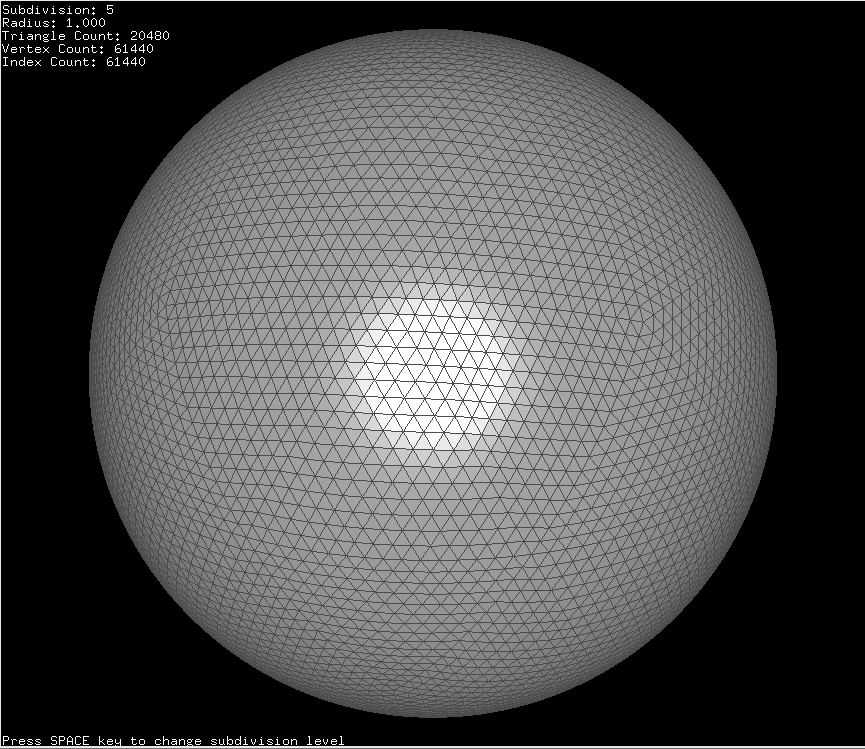
\includegraphics[width=0.49\linewidth]{img/icosphere.png} \end{center}
\caption{Affichage d'une sphère en OpenGL avec plus de 10000 polygones}
\end{figure}

\paragraph{Avantages}
    \begin{itemize}
                \item {Flexible et open source.}
                Comme les fonctionnalités de la bibliothèque sont très proche du matériel, cela permet une grande marge de manoeuvre aux développeurs pour rendre ce qu'ils veulent. Si besoin est, on peut implémenter de nouvelles fonctionnalités ou les adapter directement au sein de la bibliothèque.
                
                \item {Performant.}
                Comme justement cette bibliothèque est utilisé par de nombreuses compagnies, studio et équipes de développement afin de faire des applications graphiques en temps réel(60 FPS 4k maintenant), les performances de cette bibliothèque n'est plus à prouver.
    \end{itemize}

\paragraph{Inconvénient}
    \begin{itemize}
                \item {Complexité de prise en main.} 
                OpenGL et ses bibliothèques offrent une très grande flexibilité mais la compréhension et la prise en main de celles-ci est très complexe, comme il y en a beaucoup. Il y a cependant de bons tutoriels et une bonne documentation, mais il faudra prendre en compte l'apprentissage dans le temps passé au développement.
                
                \item {Temps de développement.}
                Du fait que OpenGL est en C/C++, pour bien organisé et réfléchir au code ça demandera du temps pour la gestion mémoire et l'architecture. Il faudra donc avoir ces faits en tête lors du développement.
                
    \end{itemize}
\newpage
\section{Besoins fonctionnels}

Les besoins sont ordonnés par ordre de priorité. A partir d'une certaine priorité, on jugera non nécessaire les fonctionnalités décrites.

\subsection{Génération procédurale d'une planète}
\begin{enumerate}

    \item\textbf{Créer la géométrie}
        \begin{itemize}
            \item {Faire le relief de la planète: repère et échelle}\\
            Afin de créer le relief de la planète, cela induit de changer "l'altitude" des sommets de la surface.
            C'est pour cela qu'il faut un repère.  Point de vue de l'implémentation, la bibliothèque de départ et son propre système de coordonnées sera un facteur important quand au choix de l'abstraction, mais en soit il existe deux possibilités :
            \begin{itemize}
                \item Un repère orthonormé.
                \item Un repère angulaire.
            \end{itemize}
            
            Pour le repère orthonormé, on peut faciliter les calculs et la représentation en utilisant comme origine du repère le centre de la planète, n'ayant pas d'autres objets à représenter sur la scène.\\
            Ce système a comme avantage d'être simple à implémenter, et d'être relativement intuitif sur la visualisation pour le déboguage.
            \\
            Une autre possibilité serait de raisonner selon des coordonnées sphériques, et une hauteur de sommet par rapport au centre, un repère angulaire couplé à une altitude. Cela a l'avantage de faciliter les calculs en cas d'applications des textures, de génération de positon des sommets, et aussi de raisonner selon un système physique de longitude et latitude. 
            Cependant il existe peu d'outils qui utilise des coordonnées radial, donc il faudra sûrement combiner les deux systèmes.\\
            
            //IMAGE DES DEUX SYSTEMES
            
            Il faut aussi fixer une unité de mesure pour la distance entre les sommets de la surface et le centre de la planète, afin de mieux pouvoir appréhender les valeur de hauteur placées des sommets, en tant que développeur. \\
            Une possibilité pour ça est de fixer un niveau fixe, comme un niveau de la mère et de raisonner à partir de celui-ci. Pour faciliter le code, on pourrait ramener l'altitude entre l'espace [-1,1], 0 étant le niveau de la mère, -1 étant l'altitude du centre de la terre. La hauteur du coup maximal est limité. Une autre façon est de ne pas faire de niveau de mer et de laisser les valeurs à partir d'une unité arbitraire. Avec ce système, il suffit de multiplier l'unité par une valeur physique pour pouvoir représenter des valeurs comparable à la réalité. On préférera ce système pour faciliter les calculs, et parce que il présente comme avantage, par rapport au premier de raisonner qu'avec des valeurs positives, qu'on peut associer à une représentation réaliste.\\
            
            \item {Créer la surface}
            Il faut définir à l'avance quel type de polygones ou type de face on va utiliser pour le maillage de la forme, qui va influencer le parcours et construction de la sphère. On a comme choix:
            \begin{itemize}
                \item{le triangle :}\\
                En l'utilisant on pourra modéliser un objet de type icosphère, un solide composé de face triangulaires. Le gros avantage de cette forme est que tous les triangles font la même taille, mais également qu'on peut augmenter le nombre de faces en sub-divisant les faces existantes (on pourra se servir de cela au moment de l'avancement du projet pour déterminer des ensembles de faces qui appartiendront à un biome). On notera également qu'elle ne présente pas de singularités aux pôles nord et sud.
                \item{le carré: cube sphère}\\
                En l'utilisant on pourra modéliser un objet "cube sphère", un solide à forme approximativement sphérique et composé de faces carrées. Elle est également sub-divisable et ne présente non plus pas de singularités aux pôles nord et sud.
                \item{le carré et le triangle: uv sphère}\\
                En les utilisant on pourra modéliser un objet "uv sphere", un solide composé composés de triangles sur les pôles, et de quadrilatères ailleurs. Il est découpé selon la longitude et la latitude. Ces faces ne sont pas de la même tailles, et aux pôles elles sont de la même forme, mais le découpage longitude-latitude fait qu'il sera plus facile de se repérer et de placer les points.
            \end{itemize}
            
        \end{itemize}
            
        \item \textbf{Renseigner des informations (données)}
            \begin{itemize}
                \item {L'objet planètaire :}\\
                Elle sera représentée sous forme d'icosphère (POURQUOI ?), un solide en trois dimensions, composé de faces triangulaires. 
                L'objet contiendra une liste de sommets, avec leurs caractéristiques que l'on définit plus bas, et une liste de caractéristique pour les faces.
                \item {Définir des propriétés de points :}\\
                Les points auront chacun une altitude par rapport au centre, qui sera généré procéduralement avec un algorithme choisi.(PEUT ETRE PLUS)
                \item {Définir des propriétés de polygones :}\\
                La caractéristiques dans la liste pour les faces devront contenir:
                    \begin{itemize}
                        \item {3 sommets,}\\
                        afin que l'on puisse retrouver le triangle à dessiner et son emplacement,
                        \item {une couleur,}\\
                        au format HSV (ou RGB selon les préférences(QUELS AVANTAGES ?)), qui sera dans un premier temps déterminée en fonction de la hauteur des points du triangle. 
                        On pourra lors de l'avancement du projet changer cela pour une application de terrains différents à la même altitude (déserts, ville, plaines, plage, taïga...)
                        \item {valeurs complémentaires :}\\
                        On pourra également y mettre des informations comme la température/le climat, la densité de population etc, qui serviront lors de la génération.
                \end{itemize}
        \end{itemize}
\end{enumerate}

\subsection{Visualisation de la planète}

\begin{enumerate}
        \item \textbf{Afficher la planète :} \\
        
        Il existe deux méthodes principales pour le rendu d'une scène 3D :
        \begin{itemize}
            \item \textbf{Rasterization}
            \item \textbf{Ray tracing}
            A COMPLETER PAR TSIORY.
        \end{itemize}
        La planète est caractérisée par une sphère aux faces polygonales, en low-poly (c'est à dire avec peu de polygone). (DANS GENERATION, A DEPLACER Chaque polygone représente une information sur la planète : un relief (hauteur des points), une couleur bleue pour l'eau, vert pour les terres, gris/marron pour les montagnes...)\\
        
        Une seule planète doit être affichée à la fois. Afin d'y parvenir, il faut donc créer une fenêtre (possiblement grâce à OpenGL). Étant donné la visée ludique de cet outil, une fenêtre carrée ou rectangulaire avec seulement la planète au centre semble être le plus approprié pour l'immersion et l'interaction avec la souris (voir figure \ref{itf_souris}, de préférence directement avec l'objet ce qui est plus ludique que l'utilisation de boutons ou de seekbar, voir figure \ref{itf_seekbar}). Pour ce faire, nous préférerons la bibliothèque open-source GLFW qui permet de gérer une fenêtre, un contexte, des évènements clavier/souris etc.\\
  
         \begin{figure}[!h]
        \begin{center} 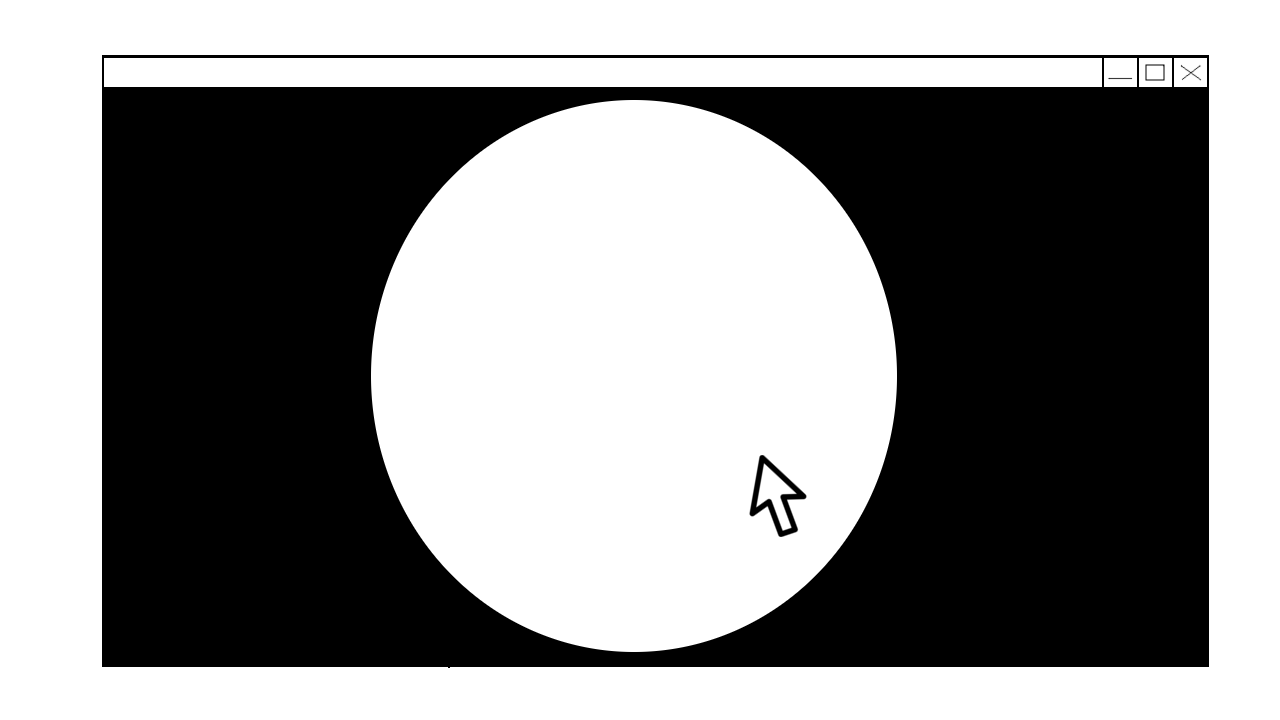
\includegraphics[width=\linewidth]{img/interface_souris.png} \end{center}
        \caption{\label{itf_souris} Prototype imagée de l'interface utilisateur}
        \end{figure}
        
        \begin{figure}[!h]
        \begin{center} 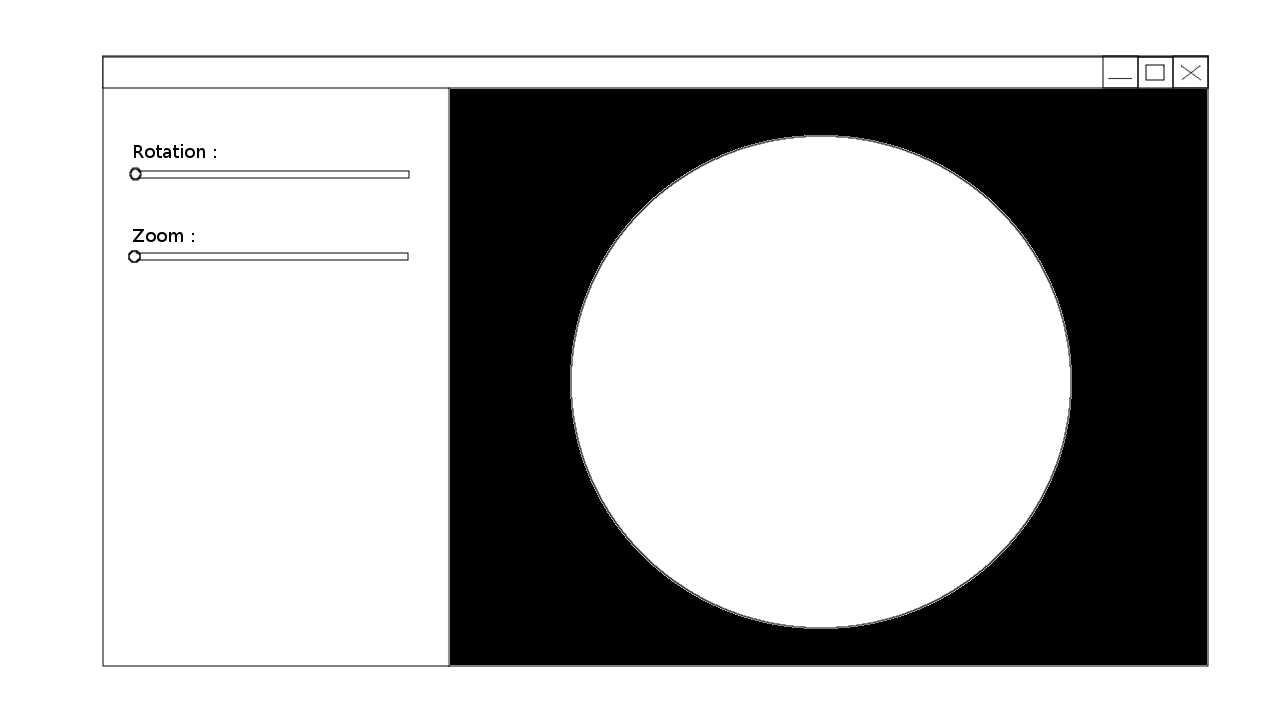
\includegraphics[width=\linewidth]{img/interface_seekbar.png} \end{center}
        \caption{\label{itf_seekbar} Prototype imagée de l'interface utilisateur avec seekbar (dépréciée)}
        \end{figure}
    
    \newpage
        \item \textbf{Effectuer une rotation du point de vue autour de la planète :} \\
        Il doit être possible de tourner, se déplacer assez précisément autour de la planète. Pour cela, un point de vue sera définit par une "caméra" qui se déplacera dans l'espace vectoriel (définit plus haut) lors d'un mouvement de la souris pendant que le clic gauche est enfoncé (une alternative faisant l'usage du clavier est envisageable). Cette caméra aura comme point d'encrage le centre de la planète. Elle effectuera donc une rotation orbitale autour de celle-ci. On affectera (si nécessaire) un coefficient de vitesse aux déplacements de la caméra afin d'assurer que l'observation soit précise et agréable. Tout cela est rendu possible par l'intermédiaire des bibliothèques open-source GLM (pour les mouvements vectoriels) et GLFW (pour la fenêtre et les évènements clavier/souris).
        
        \item \textbf{Zoom avec changement d'orientation du plan :} \\
        Il doit être possible de zoomer (respectivement dézoomer) sur la planète. Cela est faisable en rapprochant (respectivement éloignant) la caméra de la planète lors du défilement de la molette à l'aide des bibliothèques citées précédemment.\\
        Lorsque la caméra est suffisamment proche de la planète, l'angle de vue doit changer pour nous permettre de voir l'horizon. On peut alors rotater comme une tête pour observer l'environnement. L'idée serait d'empêcher le zoom lorsque l'on est au plus près de la surface de la planète, et après avoir atteint cette limite, ignorer le point d'encrage de la caméra au centre de la planète pour pouvoir orienter la caméra à notre guise et observer librement l'environnement avec les mouvements de souris pendant que le clic gauche est enfoncé. Dans cet état, la caméra peut rotater sur elle-même mais ne peut plus se déplacer. Lors d'un dézoom, la caméra reprend en compte son point d'encrage pour assurer la visualisation orbitale de la planète. Toutes ces manipulations de caméra sont réalisables en utilisant les bibliothèques open-source citées précédemment (GLM et GLFW).
        
\end{enumerate}


\subsection{Guider la génération de la planète}

Il doit être possible pour l'utilisateur de guider la génération d'une planète en passant des paramètres à notre algorithme/générateur. Ce passage de paramètres pourrait simplement se faire par ligne de commande lors de l'appel à l'exécutable. Ces paramètres influeront donc sur les transformations appliquées à la planète (plus ou moins d'altitude, de type de terrain... Par exemple, \verb|./planet -altitude 5| accentuerai d'un facteur 5 la présence de montagnes).\\
\\
Afin de réaliser ses transformations //MARC A FAIRE, ALGO DE PERLIN NOISE ETC.\\
\\
Les besoins fonctionnels qui suivent sont optionnels.

\subsection{...}


\newpage
\section{Besoins non fonctionnels}

    \begin{itemize}
    
    \item \textbf{Le programme doit pouvoir être utilisé par le client.} \\
    Le client doit pouvoir l'utiliser sur sa machine, et il faut donc s'adapter à son matériel, n'ayant pas forcément comme machine une configuration du CREMI.
    Cela induit une compatibilité \textbf{Linux}(DISTRIBUTION ET VERSION A PRECISER) et un test de performance sur une configuration proche de la machine visée. Tous les outils envisagés ont des performances variables suivant la machine envisagé, c'est donc un \textbf{point critique} à notre code.
    
    \item \textbf{Temps d'affichage minimal} \\
    Afin d'avoir une ergonomie de visualisation correct, il faut au minimum 30 image par seconde(FPS), voire plus selon la sensibilité du client. (PRECISER AVEC LE CLIENT SES ATTENTES MINIMALES).
    Un test envisageable sans le programme serait d'envoyer au client une vidéo avec les différences de FPS pour s'assurer de ce qu'il veut.
    
    \item \textbf{Rendu minimum} \\
    Il faut un certain nombre de polygones pour rendre une visualisation de la planète assez détaillé pour le client. Comme nous ne pouvons pas savoir les détails primordiaux que veut afficher le client et que c'est susceptible de changer, il faudrait que cela soit un paramètre de notre génération. Ce besoin influe de manière importante sur le temps d'affichage, il sera nécessaire de déterminer les limites du dit paramètre.
    
    \item \textbf{A voir pour ce qu'il entend par mémoire (vive-> performances et temps , dure-> sauvegarde )}
    \end{itemize}

\newpage
\section{Besoins secondaires}

\subsection{Besoins fonctionnels optionnels}
\begin{itemize}
\item \textbf{Sauvegarder les planètes générés.} \\
    L'utilisateur doit avoir la capacité de sauvegarder les modifications appliquées à une planète puis la recharger pour une utilisation ultérieure. Cette sauvegarde peut être fait en gardant les données sous un format spécifique (txt,json,yaml,xml,obj...).
    
\item \textbf{Éclairage :} \\
    Ajout d'une source de lumière à un endroit de la scène, par exemple le soleil pour la terre qui influera sur le cycle jour et nuit sur certaines parties de la planète.Sur la partie non éclairée par la lumière il fera nuit et inversement pour le jour. 
    
\item \textbf{Changer le style de visualisation} \\
    Pouvoir influer et faire des transformations sur les couleurs ou sur les ombres pour changer le style graphique.Dans un premier temps, changer la palette des couleurs peut être une amélioration optionnel facile suivant l'architecture

\item \textbf{Plusieurs biomes}\\
    Un biome de manière générale est un écosystème terrestre ou aquatique caractéristique de grandes zones biogéographiques soumises à un climat particulier. Il faut donc diversifier certaines zones de la planètes en fonction de certains paramètres comme l'altitude (montagnes, plaines), la présence aquatique (rivières,ocean), climat (nuageux,dégagé).
    
\item Quadrillage de Voronoï
\item Influence des plaques tectoniques sur le relief
\item Couches (ciel, magma, etc)
\item Se déplacer sur la surface de la planète en 1ère personne
\end{itemize}
    
\subsection{Besoins non fonctionnels optionnels}
\begin{itemize}
\item Système de fichier partagé avec l’autre groupe
\item Rendu adaptatif permettant un raffinement du rendu et de meilleurs performances

\end{itemize}

\section{Tests}

\section{Diagramme de Gantt}

\section{Annexes}


\section{Bibliographie}

\bibliographystyle{plain}

\bibliography{bibliographie}




\end{document}
